\section{Modelagem numérica de dutos submarinos}\label{chap:assentamento}


A simulação numérica do duto projetado em um ambiente tridimensional realista obtido por medições da topografia do fundo marinho, permite que os engenheiros explorem quaisquer oportunidades que o comportamento do mesmo pode oferecer para desenvolver soluções seguras e econômicas. % chktex 19
Por exemplo, o projetista pode analisar primeiro o comportamento do duto na batimetria original.
Se alguns dos casos de carga resultam em tensões além do limite aceitável, pode-se simular uma modificação do fundo do mar no modelo de elementos finitos.
A análise é executada novamente para confirmar que as modificações levaram à diminuição desejada de tensão ou deformação.

O modelo de elementos finitos pode ser uma forma para analisar o comportamento \textit{in-situ} de um duto.
Por comportamento \textit{in-situ} de um duto, entenda-se a resposta do mesmo às cargas ao longo de um histórico de carregamento~\cite{Bai2014}. Isto pode consistir em vários casos de carga em sequência, como, por exemplo:

\begin{enumerate}
    \item Instalação;
    \item Testes de pressão (enchimento de água e do teste hidrostático);
    \item Operação (enchimento com conteúdo, pressão de projeto e temperatura);
    \item Ciclos de carga/descarga;
    \item Flambagem lateral e vertical (\textit{upheaval});
    \item Onda dinâmica e/ou de corrente;
    \item Cargas de impacto.
\end{enumerate}

\citeonline{Bai2014} apresentam o processo de análise do comportamento \textit{in loco} desses dutos através do MEF, que será detalhado a seguir.

FLUXOGRAMA

\subsection{Análise estática}


A modelagem da instalação do duto é o primeiro passo para o estudo do comportamento \textit{in-situ} do duto. Visa reproduzir a configuração indeformada do duto assim que lançado sobre a leito marinho.
Essa configuração é o ponto de partida para as etapas posteriores da análise.
Mais importante do que investigar o comportamento do duto durante a instalação é garantir que a correta representação da tração e ângulo de lançamento de tal modo que consigam gerar forças residuais no duto, oriundas do atrito quando o mesmo se assenta sobre a batimetria.

Por simplicidade, neste trabalho, assume-se o ângulo entre o duto e a horizontal nulo, isto é, o duto está em um plano horizontal que desce em direção a superfície batimétrica.
Desse modo, o modelo permite especificar somente a tração de lançamento.
Essa modelagem visa garantir a correta representação do contato entre o duto e a batimetria (forças de contato e ponto onde o duto toca o solo).
A \autoref{fig:lancamentododuto} mostra o duto antes e durante o processo de instalação.

\begin{figure}[!ht]
    \centering
    \caption{Modelo de elementos finitos durante o lançamento.}\label{fig:lancamentododuto}
    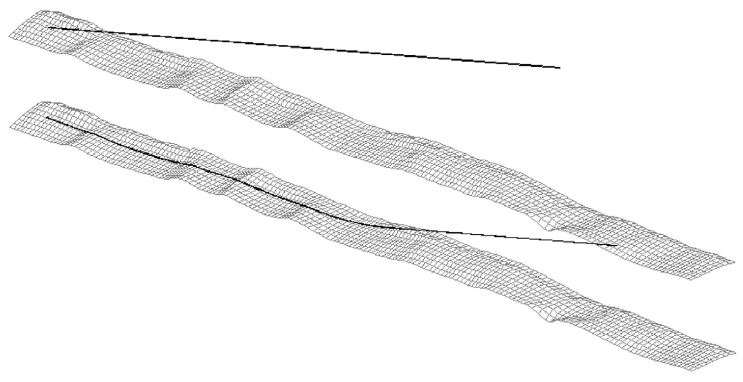
\includegraphics[width=0.7\linewidth]{imagens/lancamento_do_duto}
    \fonte{\citeonline{Bai2014}}
\end{figure}

A medida que o duto se assenta, é necessário garantir um equilíbrio estável entre ele e o solo, o que é feito mediante um modelo representativo dessa iteração, no qual deve-se definir o atrito e rigidez do leito marinho.
No ABAQUS~\cite{Dassault2018}, pode-se relacionar a penetração e a força de reação do solo por meio de uma curva de rigidez axial, além de usar modelo anisotrópico para o atrito do solo, representando as diferenças entre os atritos nas direções longitudinal e transversal.

Após a descida do duto, têm-se os processos de alagamento e desalagamento, que acarreta mudanças no peso submerso do duto e, consequentemente, altera na sua configuração.
Esses processos podem ser facilmente modelados por uma variação em uma carga vertical atuando no duto.
Mas, um duto sujeito a essa variação de carga na condição alagada sofrem grandes deformações axiais devido à mudança em geometria, e assim o duto se deforma e afunda nos vãos-livres ao longo da rota do duto.

Dessa maneira, é desejável que o modelo a ser estabelecido use um procedimento de análise que considere grandes deslocamentos e o efeito de alterações na área da seção do duto devido à alta tensão axial.
Além disso, é interessante que o modelo do material seja capaz de representar o comportamento plástico da seção do duto. No trabalho aqui proposto, não são contempladas nas análises os efeitos de carregamentos de temperatura.

A pressão hidrostática externa é um fator importante para a capacidade de resistência de duto em águas profundas.
Como o modelo pode incluir uma estrutura tridimensional no fundo do mar, a pressão externa pode ser uma função da profundidade da água.
Já a pressão interna pode ser assumida como constante, mas a possibilidade de representar o efeito estático do conteúdo na extremidade pode ser incluído.


\subsection{Procedimentos e etapas de carregamento na análise de elementos finitos}


Um conceito base no ABAQUS~é a divisão do histórico do cargamentos em etapas de carga. Para cada etapa, o usuário escolhe um método de análise.
Dessa forma, é possível representar qualquer sequência  e histórico de carregamento.
Por exemplo, em um passo estático, o duto pode ser carregado com gás, no passo estático seguinte descarregado, e na terceira etapa, pode-se realizar uma análise exclusiva do duto vazio.
Um histórico de carga de um modelo construído para uma análise de assentamento de duto é apresentado na~\autoref{tab:load_steps}.


\begin{table}[!ht]
\renewcommand{\arraystretch}{1.2}
\small
\centering
\caption{Histórico de carga típico em uma análise de dutos no ABAQUS.}\label{tab:load_steps}
\begin{tabular}{cll}
\toprule[1.5pt]

\textbf{Passo} & \textbf{Ação} & \textbf{Análise} \\
\midrule
1 & Aplicação de peso próprio e empuxo do duto & Estática \\
2 & Aplicação de pressão externa hidrostática & Estática \\
3 & Aplicação de tensão leiga & Estática \\
4 & Assentamento do duto no fundo do mar (ver \autoref{fig:lancamentododuto}) & Estática \\
5 & Remoção dos elementos de guincho & Estática \\
6 & Modificando condições de contorno para a condição de instalação & Estática \\
7 & Enchimento de água para condições alagadas & Estática \\
8 & Aplicação de pressão do teste hidrostático. & Estática \\
9 & Remoção da pressão do teste hidrostático & Estática \\
10 & Enchimento de gás & Estática \\
11 & Aplicação de pressão de operação & Estática \\
12 & Aplicação de temperatura de operação para a condição operacional & Estática \\
13 & Remoção de pressão e temperatura para condição de recarga & Estática \\
14 & Aplicação de carga de onda e corrente & Dinâmica \\

\bottomrule[1.25pt]
\end{tabular}
\\[6pt]
Fonte: \citeonline{Bai2014}.
\end{table}

Após os passos referentes aos processos de assentamento do duto, é possível incluir um passo de pertubação linear para obtenção dos modos de vibração, que são essenciais na análise de fadiga.

É válido de nota que a análise estática disponível no ABAQUS usada no modelo lida com respostas não lineares de efeitos de grandes deslocamentos, não-linearidade do material e não-linearidades de contorno, como contato, deslizamento e atrito (interação solo-duto). O ABAQUS usa o método de Newton para resolver as equações de equilíbrio não lineares. Portanto, a solução é obtida como uma série de incrementos com iterações para obter equilíbrio dentro de cada incremento~\cite{SIMULIA2018}.

\subsection{Tipos de elementos}

O ABAQUS dispõe de alguns tipos de elementos a serem usados no modelo do sistema de solo-duto com elementos finitos, conforme a \autoref{fig:elements_type}:

\begin{itemize}
    \item Para modelar o fundo do mar pode-ser usar os elementos rígidos do tipo R3D4 usados, ou superfícies analíticas rígidas.
    \item Os elementos do tipo PIPE31H usados para modelar o duto.
    \item Os elementos de molas usados para representar a continuidade do duto nas extremidades.
\end{itemize}

\begin{figure}[!ht]
    \centering
    \caption{Tipos de elementos usados no modelo.}\label{fig:elements_type}
    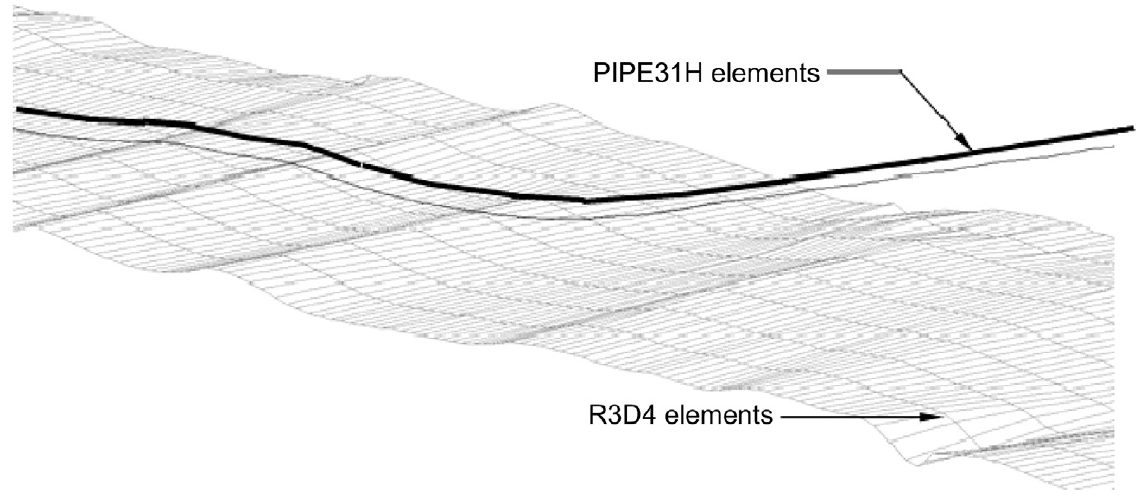
\includegraphics[width=0.8\linewidth]{imagens/elements_types}
    \fonte{\citeonline{Bai2014}}
\end{figure}

\subsubsection{Elementos para representação do duto}

A \autoref{fig:elemen_PIPE31H} mostra o elemento de duto finito 3D usado no modelo estabelecido, com 2 nós e 12 graus de liberdade.
O elemento PIPE31 usa interpolação linear, e o elemento PIPE32 interpolação quadrática.
A formulação híbrida torna o elemento adequado para casos com estruturas delgadas e problemas de contato, como um duto descendo sobre o fundo do mar.

Os elementos híbridos (PIPE31H/PIPE32H) são fornecidos para uso nos casos em que é numericamente difícil calcular as forças axiais e de cisalhamento pelo método de deslocamento próprio do Método dos Elementos Finitos.
O problema nesses casos é que pequenas diferenças em posições nodais podem causar forças muito grandes em algumas partes do modelo, o que por sua vez, causar grandes deslocamentos em outras direções.
Os elementos híbridos superam essa dificuldade usando uma formulação mais geral, na qual as forças de cisalhamento axial e transversal nos elementos são incluídas, juntamente com os deslocamentos e rotações nodais, como variáveis primárias.
Embora essa formulação torne esses elementos mais custosos computacionalmente, eles geralmente convergem muito mais rapidamente quando as rotações dos dutos são grandes.

O elemento está disponível com uma seção circular vazada de paredes finas e suporta a possibilidade de o usuário especificar pressão externa ou interna.
Elementos de paredes espessas também estão incluídos no ABAQUS\@.
O elemento também pode considerar alterações na área da seção do duto devido ao alto nível de tensão axial do duto.

\begin{figure}[!ht]
    \centering
    \caption{Elemento PIPE31.}\label{fig:elemen_PIPE31H}
    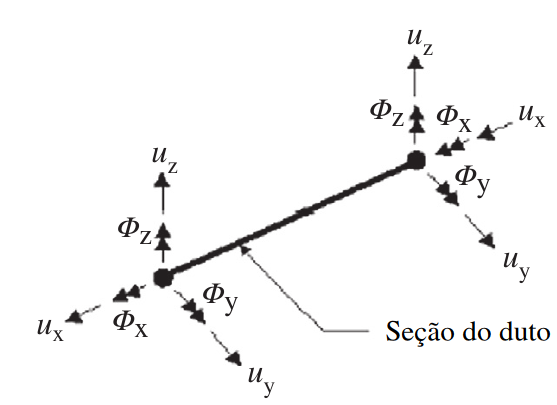
\includegraphics[width=0.5\linewidth]{imagens/elemen_PIPE31H}
    \fonte{\citeonline{Bai2014}}
\end{figure}


\subsubsection{Elementos para representação do fundo do mar}


\subsubsubsection{Elemento R3D4}


O elemento rígido R3D4 de quatro nós, como mostrado na \autoref{fig:element_R3D4}, possibilita modelar superfícies complexas com geometria arbitrária e é geralmente escolhido ao modelar a topografia do fundo do mar. Uma característica muito importante do ABAQUS ao modelar o fundo do mar tem sido a possibilidade de suavizar as superfícies geradas com os elementos rígidos, o que leva a uma representação muito melhor do fundo do mar do que a superfície facetada inicial.

\begin{figure}[!ht]
    \centering
    \caption{Elemento rígido R3D4 (a), e suavização da superfície de elementos (b).}\label{fig:element_R3D4}
    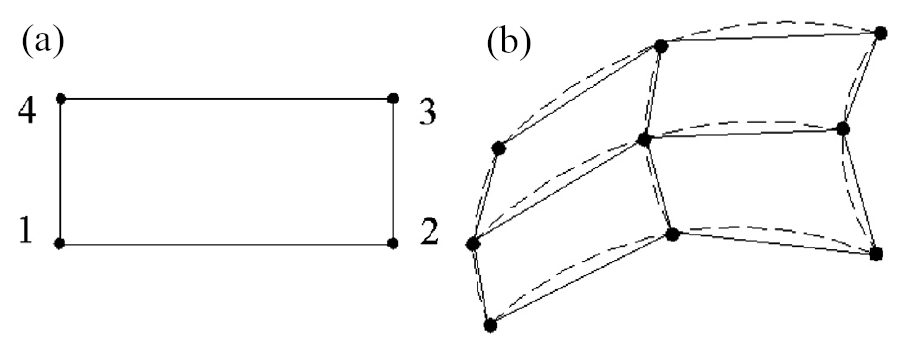
\includegraphics[width=0.7\linewidth]{imagens/element_R3D4}
    \fonte{\citeonline{Bai2014}}
\end{figure}

A suavização é feita pela ABAQUS, criando superfícies de Bèzier com base na superfície facetada do fundo do mar, formada pelos elementos rígidos. As superfícies de Bèzier resultantes, diferentemente da superfície do elemento facetado, são lisas e têm uma superfície externa com direção normal contínua. As superfícies de Bèzier não correspondem exatamente à geometria facetada da superfície rígida, mas os nós dos elementos rígidos que definem o fundo do mar permanecem sempre na superfície de Bèzier. Além disso, o usuário pode especificar o grau de suavização para controlar a geometria da superfície suavizada.

Um conjunto de elementos R3D4 que definem o fundo do mar é usado como a superfície principal chamada para aplicações de contato com os elementos do duto. Isso significa que um par de contatos (solo-duto) é definido e um modelo de interação é especificado. Esse modelo de interação geralmente consiste em uma definição de rigidez e atrito no fundo do mar.


\subsubsubsection{Superfície analítica rígida}


Outra forma de representar a batimetria do piso marinho é utilizar uma superfície analítica rígida, isto é, uma superfície geométrica com perfis que podem ser descritos com segmentos de linha reta ou curva, conforme Figura~\ref{fig:superficie_analitica}. Esses perfis podem ser varridos por um vetor gerador ou rotacionados em relação a um eixo para formar uma superfície tridimensional. Uma superfície analítica rígida está associada a um nó de referência de corpo rígido, cujo movimento governa toda a superfície. É importante frisar que este tipo de superfície possui apenas um lado disponível para contato, especificado de acordo com a orientação de eixos definida.

\begin{figure}[!ht]
    \centering
    \caption{Exemplo de superfície analítica rígida.}\label{fig:superficie_analitica}
    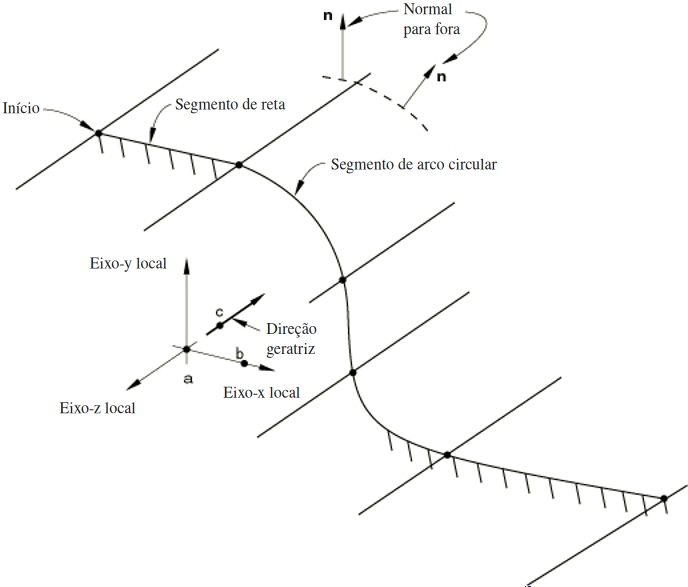
\includegraphics[width=0.7\textwidth]{imagens/superficie_analitica}
    \fonte{\citeonline{SIMULIA2018}}
\end{figure}

Em relação ao uso de superfícies formadas por elementos, o uso de superfícies analíticas rígidas apresenta duas vantagens:
\begin{itemize}
    \item Superfícies geométricas curvas podem ser modeladas com precisão, uma vez que é possível parametrizá-las com segmentos de linhas curvas, o que tem como resultado uma superfície mais suave, fornecendo uma melhor aproximação à restrição de contato físico.
    \item Menor custo computacional decorrente do algoritmo de contato.
\end{itemize}

Por outro lado, como desvantagens do uso deste tipo de superfície:
\begin{itemize}
    \item Uma superfície analítica rígida sempre agirá como superfície \textit{master} em uma interação de contato, impossibilitando que se modele o contato entre duas superfícies rígidas analíticas.
    \item Forças de contato e pressões não podem ser plotadas em uma superfície rígida analítica, apenas na superfície \textit{slave}.
    \item Um número muito grande de segmentos, na ordem de milhares, para definir uma superfície rígida analítica pode diminuir o desempenho. Sendo mais recomendável o uso de superfície baseada em elementos.
\end{itemize}


Para os casos estudados, utilizou-se uma superfície cilíndrica rígida tridimensional.
